% it/figures/data_pipeline/fig_pca_scree.tex — versione italiana
\begin{figure}[!ht]
    \centering
    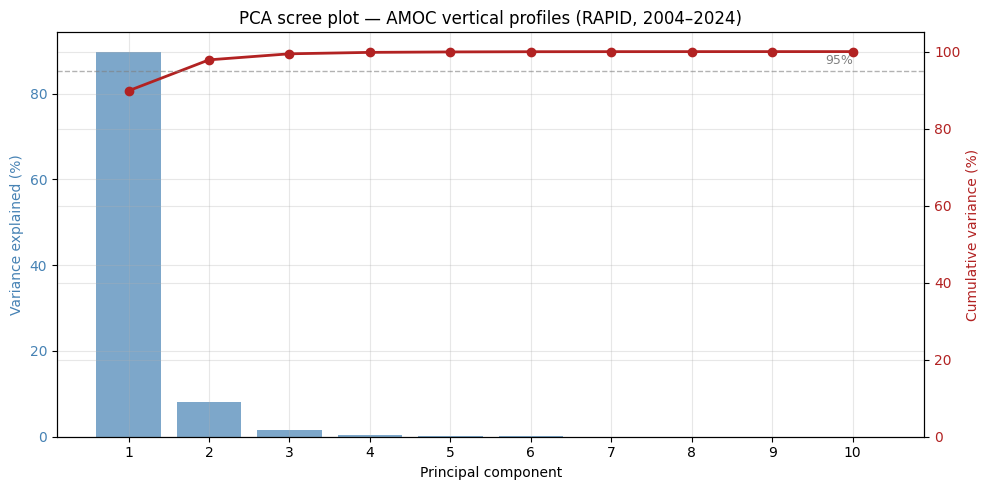
\includegraphics[width=0.8\textwidth]{figures/data_pipeline/pca_scree.png}
    \caption[Varianza spiegata dai modi PCA verticali.]{\textbf{La variabilità
    verticale dell'AMOC è quasi monodimensionale.} Varianza spiegata da ciascuna
    componente principale dei profili verticali a 307 livelli. Il primo modo da solo
    spiega il \SI{89.82}{\percent} e i primi due insieme il \SI{97.86}{\percent};
    il netto gomito dopo il secondo modo segna dove la struttura cede al rumore.
    Questo è lo spazio latente a due coordinate su cui è costruita la rappresentazione
    esperienziale.}
    \label{fig:pca-scree}
\end{figure}
